% Seven-drone scenario: cable 1 at t=7.0, cable 3 at t=12.0, cable 5 at t=14.0
% Three panels: pre-fault (t=6.0), after first fault (t=8.0), settled after all three (t=18.0)
% XY-plane relative positions (drone - load)
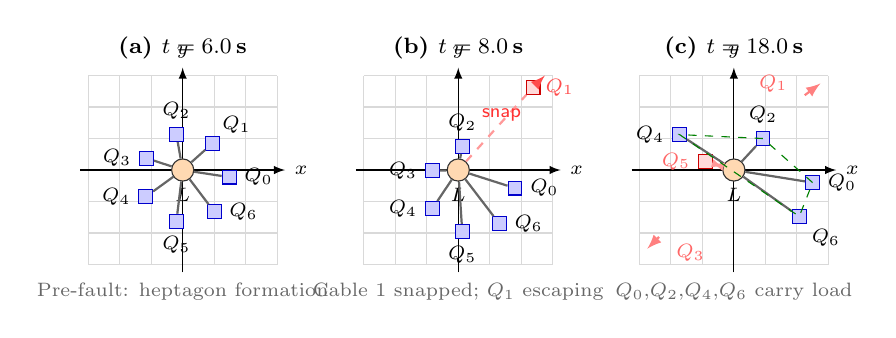
\begin{tikzpicture}[
  drone/.style={draw=blue!80!black, fill=blue!20, minimum size=5pt, inner sep=0pt, font=\tiny},
  faulted/.style={draw=red!80!black, fill=red!15, minimum size=5pt, inner sep=0pt, font=\tiny},
  payload/.style={circle, draw=black!80, fill=orange!30, minimum size=8pt, inner sep=0pt},
  cable/.style={thick, black!60},
  snapped/.style={thick, red!40, dashed},
  panel/.style={font=\footnotesize\bfseries},
  lbl/.style={font=\scriptsize},
  >=latex
]

% === Panel (a): t = 6.0 s — Pre-fault ===
\begin{scope}[shift={(0,0)}]
  \draw[gray!30, thin] (-1.2,-1.2) grid[step=0.4] (1.2,1.2);
  \draw[->] (-1.3,0) -- (1.3,0) node[right, font=\scriptsize]{$x$};
  \draw[->] (0,-1.3) -- (0,1.3) node[above, font=\scriptsize]{$y$};

  % Payload at origin
  \node[payload] (L) at (0,0) {};
  \node[lbl, below=3pt] at (L) {$L$};

  % Drone positions relative to load at t=6.0
  % D0: (2.587-2.000, 1.003-1.093) = (0.587, -0.090)
  % D1: (2.384-2.000, 1.435-1.093) = (0.384, 0.342)
  % D2: (1.919-2.000, 1.545-1.093) = (-0.081, 0.452)
  % D3: (1.537-2.000, 1.247-1.093) = (-0.463, 0.154)
  % D4: (1.535-2.000, 0.750-1.093) = (-0.465, -0.343)
  % D5: (1.922-2.000, 0.446-1.093) = (-0.078, -0.647)
  % D6: (2.398-2.000, 0.560-1.093) = (0.398, -0.533)
  \node[drone] (D0) at ( 0.59, -0.09) {};
  \node[drone] (D1) at ( 0.38,  0.34) {};
  \node[drone] (D2) at (-0.08,  0.45) {};
  \node[drone] (D3) at (-0.46,  0.15) {};
  \node[drone] (D4) at (-0.47, -0.34) {};
  \node[drone] (D5) at (-0.08, -0.65) {};
  \node[drone] (D6) at ( 0.40, -0.53) {};

  % Cables
  \foreach \d in {D0,D1,D2,D3,D4,D5,D6} {\draw[cable] (L) -- (\d);}

  % Labels (positioned to avoid overlap)
  \node[lbl, right=2pt] at (D0) {$Q_0$};
  \node[lbl, above right=0pt] at (D1) {$Q_1$};
  \node[lbl, above=2pt] at (D2) {$Q_2$};
  \node[lbl, left=2pt] at (D3) {$Q_3$};
  \node[lbl, left=2pt] at (D4) {$Q_4$};
  \node[lbl, below=2pt] at (D5) {$Q_5$};
  \node[lbl, right=2pt] at (D6) {$Q_6$};

  \node[panel] at (0, 1.55) {(a) $t = 6.0$\,s};
  \node[lbl, text=black!60] at (0, -1.55) {Pre-fault: heptagon formation};
\end{scope}

% === Panel (b): t = 8.0 s — 1 s after first fault (cable 1) ===
\begin{scope}[shift={(3.5,0)}]
  \draw[gray!30, thin] (-1.2,-1.2) grid[step=0.4] (1.2,1.2);
  \draw[->] (-1.3,0) -- (1.3,0) node[right, font=\scriptsize]{$x$};
  \draw[->] (0,-1.3) -- (0,1.3) node[above, font=\scriptsize]{$y$};

  % Payload at origin
  \node[payload] (L) at (0,0) {};
  \node[lbl, below=3pt] at (L) {$L$};

  % Drone positions relative to load at t=8.0
  % D0: (3.156-2.432, 0.937-1.169) = (0.724, -0.232)
  % D1: (4.045-2.432, 3.168-1.169) = (1.613, 1.999) -- escaping, off scale
  % D2: (2.486-2.432, 1.469-1.169) = (0.054, 0.300)
  % D3: (2.100-2.432, 1.161-1.169) = (-0.332, -0.008)
  % D4: (2.105-2.432, 0.681-1.169) = (-0.327, -0.488)
  % D5: (2.486-2.432, 0.385-1.169) = (0.054, -0.784)
  % D6: (2.955-2.432, 0.490-1.169) = (0.523, -0.679)
  \node[drone] (D0) at ( 0.72, -0.23) {};
  \node[drone] (D2) at ( 0.05,  0.30) {};
  \node[drone] (D3) at (-0.33, -0.01) {};
  \node[drone] (D4) at (-0.33, -0.49) {};
  \node[drone] (D5) at ( 0.05, -0.78) {};
  \node[drone] (D6) at ( 0.52, -0.68) {};

  % D1 escaping
  \node[faulted] (D1) at (0.95, 1.05) {};
  \draw[->, red!70, thick] (D1) -- ++(0.15, 0.15);

  % Cables
  \draw[cable] (L) -- (D0);
  \draw[snapped] (L) -- (D1);
  \draw[cable] (L) -- (D2);
  \draw[cable] (L) -- (D3);
  \draw[cable] (L) -- (D4);
  \draw[cable] (L) -- (D5);
  \draw[cable] (L) -- (D6);

  \node[font=\scriptsize, red!80] at (0.55, 0.70) {\textsf{snap}};

  % Labels
  \node[lbl, right=2pt] at (D0) {$Q_0$};
  \node[lbl, right=1pt, red!70] at (D1) {$Q_1$};
  \node[lbl, above=2pt] at (D2) {$Q_2$};
  \node[lbl, left=2pt] at (D3) {$Q_3$};
  \node[lbl, left=2pt] at (D4) {$Q_4$};
  \node[lbl, below=2pt] at (D5) {$Q_5$};
  \node[lbl, right=2pt] at (D6) {$Q_6$};

  \node[panel] at (0, 1.55) {(b) $t = 8.0$\,s};
  \node[lbl, text=black!60] at (0, -1.55) {Cable 1 snapped; $Q_1$ escaping};
\end{scope}

% === Panel (c): t = 18.0 s — Settled after all 3 faults ===
\begin{scope}[shift={(7.0,0)}]
  \draw[gray!30, thin] (-1.2,-1.2) grid[step=0.4] (1.2,1.2);
  \draw[->] (-1.3,0) -- (1.3,0) node[right, font=\scriptsize]{$x$};
  \draw[->] (0,-1.3) -- (0,1.3) node[above, font=\scriptsize]{$y$};

  % Payload at origin
  \node[payload] (L) at (0,0) {};
  \node[lbl, below=3pt] at (L) {$L$};

  % Drone positions relative to load at t=18.0
  % D0: (-1.510-(-2.514), 0.837-0.994) = (1.004, -0.157)
  % D1: escaped far (6.5, 5.3)
  % D2: (-2.141-(-2.514), 1.391-0.994) = (0.373, 0.397)
  % D3: escaped far (-3.4, -0.7)
  % D4: (-3.199-(-2.514), 1.439-0.994) = (-0.685, 0.445)
  % D5: escaped (-2.872-(-2.514), 1.108-0.994) = (-0.358, 0.114) -- nearby still
  % D6: (-1.686-(-2.514), 0.408-0.994) = (0.828, -0.586)

  % Healthy drones: 0, 2, 4, 6
  \node[drone] (D0) at ( 1.00, -0.16) {};
  \node[drone] (D2) at ( 0.37,  0.40) {};
  \node[drone] (D4) at (-0.69,  0.45) {};
  \node[drone] (D6) at ( 0.83, -0.59) {};

  % Faulted drone 5 still nearby (marginal separation)
  \node[faulted] (D5) at (-0.36, 0.11) {};

  % Cables to surviving drones
  \draw[cable] (L) -- (D0);
  \draw[cable] (L) -- (D2);
  \draw[cable] (L) -- (D4);
  \draw[cable] (L) -- (D6);

  % Off-screen escaped drones
  \draw[->, red!50, thick, dashed] (0.90, 0.95) -- (1.10, 1.10);
  \node[lbl, red!60] at (0.50, 1.10) {$Q_1$};
  \draw[->, red!50, thick, dashed] (-0.95, -0.85) -- (-1.10, -1.00);
  \node[lbl, red!60] at (-0.55, -1.05) {$Q_3$};

  % D5 marginal separation annotation
  \node[lbl, red!60, left=2pt] at (D5) {$Q_5$};
  \draw[red!40, thin, <->] (D5) -- (L);

  % Labels
  \node[lbl, right=2pt] at (D0) {$Q_0$};
  \node[lbl, above=2pt] at (D2) {$Q_2$};
  \node[lbl, left=2pt] at (D4) {$Q_4$};
  \node[lbl, below right=1pt] at (D6) {$Q_6$};

  % Quadrilateral annotation
  \draw[green!50!black, thin, dashed] (D0.center) -- (D2.center) -- (D4.center) -- (D6.center) -- cycle;

  \node[panel] at (0, 1.55) {(c) $t = 18.0$\,s};
  \node[lbl, text=black!60] at (0, -1.55) {$Q_0$,$Q_2$,$Q_4$,$Q_6$ carry load};
\end{scope}

\end{tikzpicture}
